\documentclass[12pt,a4paper]{article} 
\usepackage{tikz}
\usepackage{float}
\usepackage{graphicx}
\usepackage{multirow}
\usepackage{setspace} 
\usepackage{graphicx}
\usepackage{times}
\pagenumbering{roman}
\usepackage{geometry}

\geometry{verbose,tmargin=2cm,bmargin=2cm,lmargin=3cm,rmargin=2cm}
\usepackage{fancyhdr} 
%\linespread{1.05} 
\usepackage{tikz}
\usetikzlibrary{arrows}
\usetikzlibrary{shapes.geometric}

\tikzstyle{kres} = [rectangle, rounded corners, minimum width=1cm, minimum height=0.5cm,text centered, draw=black]
\tikzstyle{nad} = [trapezium, trapezium left angle=60, trapezium right angle=100, minimum width=1cm, minimum height=0.5cm, text centered, draw=black]
\tikzstyle{sim} = [trapezium, trapezium left angle=60, trapezium right angle=100, minimum width=1cm, minimum height=0.5cm, text centered, draw=black]
\tikzstyle{garis} = [thick,->,>=stealth]
\usetikzlibrary{shapes,arrows}

\begin{document} % Mulai Penulisan Laporan
\onehalfspacing
\begin{titlepage}

\title{\textbf{LAPORAN PRAKTIKUM ELEKTRONIKA DASAR
\\ RANGKAIAN RC DAN FLIP FLOP }}  %Judul Laporan
%\title{\textbf{FOTOKATALISIS}}  %Judul Laporan
\author{\textbf {Dosen : Mada Sanjaya WS, Ph.D }
\\ \textbf{Asisten Lab : Noer Ardiansyah Laksana (1177030025)}
\\ \textbf{ }
\\ \textbf{Disusun Oleh :}
\\ \textbf{Muhamad Fahmi Adzkar} \textbf {(1187030024)}
\\ \textbf{Kelompok 3 :}
\\ \textbf{Hani Hikmawati} \textbf {(1187030014)}
\\ \textbf{Sri Rahayu} \textbf {(1187030036)}
\\ \textbf{Yuni Rahayu} \textbf {(1187030041)}}

\maketitle
\begin{center}
\vspace{1cm}

\includegraphics[width=4cm]{uin.png}
\vspace{1cm}

JURUSAN FISIKA\\
FAKULTAS SAINS DAN TEKNOLOGI\\
UIN SUNAN GUNUNG DJATI BANDUNG\\
2019\\
\end{center}
\end{titlepage}

\renewcommand\abstractname{Abstract} %Untuk Abstrak Bahasa Inggris
\begin{abstract}
Alhamdulillah in this day we will practice about Resistor and Capacitor Sirkuit, Flip Flop Analog.
The working principle of the flip flop circuit compared to the principle of the working of the transistor as a switch is the same, that is, if the circuit is given a voltage then one of the conditions of the transistor comes to life. This situation also has a dependency on capacitors which have higher charge heights when compared to other components. When more detailed, a capacitor with a higher charge level will cause the discharge of the electric charge first then a connection will occur between the legs of the transistor and the capacitor whose condition is on.

\subparagraph{ }
\textit{Keywords: Ohms law, Resistor and Capacitor circuit, obstacle,voltage,electric current, IC NE555.}

\end{abstract}

\renewcommand\abstractname{Abstrak} %Untuk Abstrak Bahasa Indonesia
\begin{abstract}
alhamdulillah pada percobaan kali ini kita melakukan percobaan untuk RANGKAIAN RC DAN FLIP FLOP.
Prinsip kerja dari rangkaian flip flop dibandingkan dengan prinsip dari kerja transistor sebagai saklar adalah sama, yaitu apabila rangkaiannya diberi tegangan maka salah-satu dr kondisi transistornya menjadi hidup. Keadaan ini pula memiliki ketergantungan kepada kapasitor yang memiliki ketinggian muatan yang lebih jika dibandingkan dengan komponen lainnya. Bila lebih diperinci lagi, sebuah kapasitor yang ketinggian muatannya lebih akan menyebabkan lepasnya muatan listrik lebih dulu kemudian terjadi hubungan antara kaki transistor dengan kapasitor yg kondisinya sedang on.

\subparagraph{ }
\textit{Kata Kunci: Hukum ohm, rangkaian resistor dan kapasitor, hambatan, tegangan, arus listrik, IC NE555.}

\end{abstract}

\newpage
\section{PENDAHULUAN}
\paragraph{1.1 Latar Belakang}
\subparagraph{ }
	Dalam sebuah rangkaian listrik dikenal dengan istilah arus listrik (I), tegangan atau beda potensial (V) dan hambatan (R). Pada dasarnya sebuah rangkaian listrik terjadi ketika sebuah penghantar mampu dialiri electron bebas secara terus menerus. Aliran inilah yang disebut dengan arus. Sedangkan tegangan adalah beda potensial yang ada di antara titik rangkaian listrik tersebut. Untuk menemukan hubungan di antara istilah-istilah yang ada dalam sebuah rangkaian listrik diperlukan sebuah praktikum yang dapat membuktikannya.
\subparagraph{ }
	Dengan melakukan praktikum yang berjudul RANGKAIAN RC DAN FLIP FLOP ini kita dapat mengetahui dan mempelajari hubungan antara tegangan atau beda potensial dan kuat arus pada suatu rangkaian RC (seri dan pararel)dan dapat digunakan untuk mengetahui sebuah hambatan listrik tanpa harus menggunakan alat (multimeter). Selain itu materi tentang RANGKAIAN RC DAN FLIP FLOP ini sangat berguna khususnya yang mendalami kelistrikan. Dan juga hukum ohm ini sangat berhubungan dengan alat-alat otomatis yang terjadi disekitar kita, salah satunya sensor cahaya atau Light Dependent Resistor (LDR) yang sangat bermanfaat bagi kehidupan manusia.
 
 

\paragraph{1.2 Tujuan}
\subparagraph{ }
Adapun tujuan dilakukannya praktikum ini yaitu:
\begin{enumerate}
\item Memahami fungsi rangkaian RC dan IC 555 sebagai timer.
\item Memahami dan dapat membuat rangkaian RC dan flip flop analaog.
\item Memahami prinsip kerja rangkaian RC dan flip flop analog.
\item Menganalisis hasil percobaan alat dengan simulasi.
\end{enumerate}


\newpage
\section{Landasan Teori}
\subsection{Dasar Teori}
\paragraph{ }
\textbf{Resistor Dan Kapasitor}
\subparagraph{ }
	Kondensator atau kapasitor adalah sistem konduktor yang mampu menyimpan rapat (to condense) muatan listrik sehingga memiliki daya tampung, yaitu kapasitas yang besar sehingga disebut kapasitas nya besar. Pada dasarnya kapasitas kondensator dihitung dengan merumuskan beda potensial antara kedua bagian kondesator oleh muatan listrik. V diperoleh dari rumus q = CV atau C = q/v. Agar V mudah dirumuskan, dipilihlah bentuk-bentuk geometris yang sederhana bagi kedua konduktor kondensator itu, dan dikenallah tiga macam kondesator yakni apa yang dikenal sebagai kodesator-kondesator keping, bola, dan silinder, tergantung bentuk konduktor-konduktornya.
\begin{flushright}
(Soedojo, 2004 hal: 171) 
\end{flushright}

\subparagraph{ }
	\begin{figure}
	
	\end{figure}
	Kapasitor berkapasitansi C awalnya tidak bermuatan. Untuk mengisi muatannya, kita tutup sakelar S pada titik A . Ini akan menghasilkan sebuah rangkaian seri RC yang terdiri dari kapasitor, baterai ideal dengan ggl , dan resistasi R .Kita tahu bahwa ketika rangkaian terbentuk, muatan mulai mengalir (ada arus) antara salah satu pelat kapasitor dan salah satu terminal baterai setiap sisi kapasitor. Arus ini meningkatkan muatan q pada pelat-pelat dan beda potensial (Vc = q/c ) pada kapasitor. Ketika benda potensial itu sama dengan beda potensial pada baterai, arus akan nol. Disini kita ingin mengetahui proses pengisian muatan. Secara khusus, kita ingin tahu bagaimana muatan q(t) pada pelat kapasitor, beda potensial Vc(t) pada kapasitor, dan arus i(t) pada rangkaian berubah terhadap waktu selama proses pengisian muatan. Kita mulai dengan menerapkan aturan-aturan loop pada rangkaian, melintasinya searah jarum jam dari terminal negatif baterai.
\begin{flushright}
(Haliday, 2010 hal: 179) 
\end{flushright}

\paragraph{ }
\textbf{ }
\subparagraph{ }
	\paragraph{ }
\textbf{Rangkaian Flip Flop}
\subparagraph{ }
	Rangkaian Flip Flop merupakan rangkaian yg memakai trigger, karenanya akan menghasilkan angka logic berupa 1 dan 0 disaat keluarnya. Keadaan ini terjadi karena pengaruh apabila keduanya ataupun salah satu dari angka tersebut dimasukkan. Kapasiatasnya sendiri adalah satu bit. Namun hal ini hanya berlaku apabila salah satu dr daya mereka masing terhubung ataupun terpasang. Rangkaian Flip Flop bila dibandingkan dengan fungsi dari gerbang logic dasar serta kombinasi adalah sangat jauh berbeda. Penyebabnya adalah karena keluaran dr flip flop itu sering menggantung di keadaan awal. Keadaan ini dapat juga bisa menjadikan keluarannya menjadi kondisi memory atau tidak berubah keluarannya. Nah inilah yang menjadi penyebab kenapa flip flop itu lebih sering dipakai untuk elemen memori.

\begin{flushright}
	(Soedojo, 2004 hal: 171) 
\end{flushright}

\subparagraph{ }
	Prinsip kerja dari rangkaian flip flop dibandingkan dengan prinsip dari kerja transistor sebagai saklar adalah sama, yaitu apabila rangkaiannya diberi tegangan maka salah-satu dr kondisi transistornya menjadi hidup. Keadaan ini pula memiliki ketergantungan kepada kapasitor yang memiliki ketinggian muatan yang lebih jika dibandingkan dengan komponen lainnya. Bila lebih diperinci lagi, sebuah kapasitor yang ketinggian muatannya lebih akan menyebabkan lepasnya muatan listrik lebih dulu kemudian terjadi hubungan antara kaki transistor dengan kapasitor yg kondisinya sedang on.
	Untuk merubah memory yg ada pada flip flop, kita harus memberikan clock pd masukan-nya. Rangkaian dasar yg berupa latch lah yang sebenarnya menjadi penyusun flip flop. Untuk jenis latch yg digunakan adalah memakai jenis latch – RS. Jenis latch tersebut digunakan karena bisa dibentuk dr gerbang logic NOR dan NAND. Berbeda dengan fungsi awalnya yg sangat tergantung dengan kondisi tertentu. Keadaan ini juga yg mengakibatkan tidak berubahnya keluaran.
	Semua transistor yg keadaannya masih on menjadikan kapasitor tersambung dgn kaki kolektron dan akhirnya diisi dengan muatan. Namun bila hanya salah satu transistor saja yang on, maka transistor lainnya akan menjadi off. Reaksi tersebut akan terus menerus terjadi dengan berganti-gantian yang menyebabkan aliran lampu yang menyala, yang kita sebut sebagai rangkaian flip flop.
	Sebuah flip-flop merupakan multivibrator-dwistabil. Sirkuit dapat dibuat untuk mengubah arus dengan sinyal yang dimasukkan pada satu atau lebih input kontrol dan akan memiliki satu atau dua output. Ini merupakan elemen penyimpanan dasar pada Logika Sekuensial. Flip-flop dan latch merupakan bangunan penting dalam sistem elektronik digital yang digunakan pada komputer, komunikasi dan tipe lain dari sistem.
	Flip-flop dan latch digunakan sebagai elemen penyimpan data, seperti penyimpan data yang dapat digunakan untuk menyimpan memori, seperti sirkuit yang dijelaskan pada logika sekuensial. Ketika menggunakan Read-only Memory, output dan keadaan selanjutnya tidak hanya bergantung pada input awalnya saja, namun pula pada keadaan yang sekarang. Flip-flops juga dapat digunakan untuk menghitung detak, dan untuk mengsinkronisasikan input signal waktu variable untuk beberapa signal waktu yang direferensi.

\begin{flushright}
	(Haliday, 2010 hal: 179)
\end{flushright}

\newpage
\section{METODE PRAKTIKUM}
\subsection{Waktu dan Tempat}
\paragraph{ }
Praktikum ini dilaksanakan pada:
\\ 		Tanggal : jum'at, 27 September 2019
\\ 		Waktu : 07.00 WIB - Selesai
\\ 		Tempat : Advance Physics 

\subsection{Alat dan Bahan}
Alat dan bahan yang digunakan dalam praktikum ini diantaranya adalah : 
\subparagraph*{ }
\begin{tabular}{|l|l|l|}  \hline
No & Alat dan Bahan  & Jumlah  \\ \hline
1  & Project Board & 1 Buah \\ \hline
2  & Kabel Penghubung & Secukupnya \\ \hline
3  & Resistor & Secukupnya \\ \hline
4  & Kapasitor & Secukupnya \\ \hline
5  & LED & Secukupnya \\ \hline
6  & Push Button & Secukupnya \\ \hline
7  & Resistor & Secukupnya \\ \hline
8  & Stop Watch & Secukupnya \\ \hline
9  & Soket IC 8 pin & Secukupnya \\ \hline
10  & IC NE555 & Secukupnya \\ \hline
11 & Baterai 9V dan kancingnya & 1 Set \\ \hline
12 & Multimeter & 1 Buah \\ \hline
13 & Personal Komputer / software TinkerCAD & 1 Set \\ \hline

\end{tabular}

  
    
\subsection{Prosedur Percobaan}
	\subparagraph{3.3.1 Percobaan Rangkaian RC}
	\subparagraph{ }
\textbf{Rangkaian RC} Rangkaian disusun sesuai dengan gambar simulasi di software TinkerCAD dan project board. Kemudian nilai resistansinya resistor-resistor tersebut ditentukan sendiri oleh Multimeter. Dilanjut dengan diukurnya besar resistansi total pada rangkaian dan ketika diberikan tegangan sebesar 9 V arus DC oleh Baterai,Pastikan rangkaiannya tersambung dengan benar. Diukur besar tegangan masing-masing resistor dan dijumlahkan kemudian dibandingkan dengan V sumber. Kemudian diukur besar arus yang mengalir pada rangkaian. Dihitung nilai resistansi total tegangan pada masing-masing resistor dan arus yang mengalir pada rangkaian dengan menggunakan rumus pada hukum ohm. kemudian data ditulis pada tabel dan analisi apa yang terjadi.

	\subparagraph{3.3.2 Percobaan Rangkaian Flip Flop Analog}
	\subparagraph{ }
\textbf{Rangkaian Flip Flop Analog} Disusun rangkaian seperti gambar simulasi di software TinkerCAD dan project board. Kemudian nilai resistansinya resistor-resistor tersebut ditentukan sendiri oleh Multimeter. Kemudian diukur besar resistansi pada rangkaian. Lalu tegangan diberikan sebesar 9 V arus DC oleh Baterai, Pastikan rangkaiannya tersambung dengan benar. Kemudian diukur besar tegangan pada rangkaian, diukur nilai resistansi, arus pada masing-masing resistor, dan tegangan pada rangkaian dengan menggunakan rumus pada hukum ohm  pada rangkaian tersebut. Lalu ditulis data pada tabel dan analisis apa yang terjadi.

	\subparagraph{3.3.3 Percobaan Rangkaian Flip Flop Analog Menggunakan IC NE555}
	\subparagraph{ }
\textbf{Rangkaian Flip Flop Analog Menggunakan IC NE555} Disusun rangkaian seperti gambar simulasi di software TinkerCAD dan project board. Kemudian nilai resistansinya resistor-resistor tersebut ditentukan sendiri oleh Multimeter. Kemudian diukur besar resistansi pada rangkaian. Lalu tegangan diberikan sebesar 9 V arus DC oleh Baterai, Pastikan rangkaiannya tersambung dengan benar. Kemudian diukur besar tegangan pada rangkaian, diukur nilai resistansi, arus pada masing-masing resistor, dan tegangan pada rangkaian dengan menggunakan rumus pada hukum ohm  pada rangkaian tersebut. Lalu ditulis data pada tabel dan analisis apa yang terjadi.

\subsection{Diagram Alir}
\subsubsection{Percobaan Rangkaian RC}
\tikzstyle{line} = [draw, -latex']
\tikzstyle{cloud} = [draw, rectangle,fill=blue!20, node distance=3cm,
    minimum height=0.7cm]
\tikzstyle{kres} = [draw, rectangle, rounded corners,fill=blue!20, node distance=3cm,
    minimum height=0.7cm]
\begin{tikzpicture}[node distance = 1.3cm, auto]
    % Place nodes
       \node [kres] (a) {Buat simulasi pada software TinkerCAD dan project board};
        \node [cloud, below of = a , node distance = 1.5cm] (b) {Susun rangkaian sesuai dengan gambar simulasi};         
        \node [cloud, below of = b , node distance = 1.5cm] (c) {Ukur resistansi tiap resistor dan Rtotal};
        \node [cloud, below of = c , node distance = 1.5cm] (d) {Masukan tegangan Baterai 9 Volt DC};
         \node [cloud, below of = d , node distance = 1.5cm] (e) {Mengukur dengan Multimeter};        
        \node [cloud, below of = e , node distance = 1.5cm] (f) {Bandingkan dengan simulasi};
        \node [cloud, below of = f , node distance = 1.5cm] (g) {Mengukur besar I};
        \node [kres, below of = g , node distance = 1.5cm] (h) {Hasil data ditulis pada tabel};
        \node [kres, below of = h , node distance = 1.5cm] (i) {Analisis apa yang terjadi};
        
     % Draw edges
    \path [line] (a) -- (b);
    \path [line] (b) -- (c);
    \path [line] (c) -- (d);
    \path [line] (d) -- (e);
    \path [line] (e) -- (f);
    \path [line] (f) -- (g);
    \path [line] (g) -- (h);
    \path [line] (h) -- (i);
    \end{tikzpicture}   


\subsubsection{Percobaan Rangkaian Flip Flop Analog}
\tikzstyle{line} = [draw, -latex']
\tikzstyle{cloud} = [draw, rectangle,fill=blue!20, node distance=3cm,
    minimum height=0.7cm]
\tikzstyle{kres} = [draw, rectangle, rounded corners,fill=blue!20, node distance=3cm,
    minimum height=0.7cm]
\begin{tikzpicture}[node distance = 1.3cm, auto]
    % Place nodes
       \node [kres] (a) {Buat simulasi pada software TinkerCAD dan project board};
        \node [cloud, below of = a, node distance = 1.5cm] (b) {Susun rangkain seperti pada hasil gambar simulasi};         
        \node [cloud, below of = b, node distance = 1.5cm] (c) {Tentukan nilai resistansi resistor};
        \node [cloud, below of = c, node distance = 1.5cm] (d) {Mengukur dengan Multimeter};        
        \node [cloud, below of = d, node distance = 1.5cm] (e) {Masukan tegangan Baterai 9 Volt DC};
        \node [cloud, below of = e, node distance = 1.5cm] (f) {Mengukur I pada masing-masing R};
         \node [cloud, below of = f, node distance = 1.5cm] (g) {Ukur besar tegangan pada rangkaian};
        \node [kres, below of = g , node distance = 1.5cm] (h) {Hasil data ditulis pada tabel};
         \node [kres, below of = h , node distance = 1.5cm] (i) {Analisis apa yang terjadi};
     % Draw edges
    \path [line] (a) -- (b);
    \path [line] (b) -- (c);
    \path [line] (c) -- (d);
    \path [line] (d) -- (e);
    \path [line] (e) -- (f);
    \path [line] (f) -- (g);
    \path [line] (g) -- (h);
    \path [line] (h) -- (i);
    \end{tikzpicture}
    
    \subsubsection{Percobaan Rangkaian Flip Flop Analog Menggunakan IC NE555}
\tikzstyle{line} = [draw, -latex']
\tikzstyle{cloud} = [draw, rectangle,fill=blue!20, node distance=3cm,
    minimum height=0.7cm]
\tikzstyle{kres} = [draw, rectangle, rounded corners,fill=blue!20, node distance=3cm,
    minimum height=0.7cm]
\begin{tikzpicture}[node distance = 1.3cm, auto]
    % Place nodes
       \node [kres] (a) {Buat simulasi pada software TinkerCAD dan project board};
        \node [cloud, below of = a, node distance = 1.5cm] (b) {Susun rangkain seperti pada hasil gambar simulasi};         
        \node [cloud, below of = b, node distance = 1.5cm] (c) {Tentukan nilai resistansi resistor};
        \node [cloud, below of = c, node distance = 1.5cm] (d) {Menyiapkan IC NE555};        
        \node [cloud, below of = d, node distance = 1.5cm] (e) {Masukan tegangan Baterai 9 Volt DC};
        \node [cloud, below of = e, node distance = 1.5cm] (f) {Mengukur I pada masing-masing R};
         \node [cloud, below of = f, node distance = 1.5cm] (g) {Ukur besar tegangan pada rangkaian};
        \node [kres, below of = g , node distance = 1.5cm] (h) {Hasil data ditulis pada tabel};
         \node [kres, below of = h , node distance = 1.5cm] (i) {Analisis apa yang terjadi};
     % Draw edges
    \path [line] (a) -- (b);
    \path [line] (b) -- (c);
    \path [line] (c) -- (d);
    \path [line] (d) -- (e);
    \path [line] (e) -- (f);
    \path [line] (f) -- (g);
    \path [line] (g) -- (h);
    \path [line] (h) -- (i);
    \end{tikzpicture}

\newpage

\section{Data dan Pembahasan}

\subsection{Data Hasil Pengamatan}
\paragraph{ } Setelah melakukan eksperimen, maka didapatkan hasil percobaan sebagai berikut.

\subparagraph*{$\bullet$ Kapasitor Biasa }
\subparagraph*{ }
\begin{tabular}{|c|c|c|c|c|c|c|c|c|c|c|}        \hline
No & R (Ohm) & C (Farad) & t (pengisian) & t (pengosongan) & V masuk & V keluar \\ \hline 
1. & 1 K  & 1 mikro & 1,4 s & 2,0 s & 1,5 V & 2,99 mV \\ \hline
2. & 2 K & 1 mikro & 1,1 s & 0,9 s & 1,5 V & 2,99 mV \\ \hline
3. & 100 K  & 1 mikro & 2,0 s & 2,8 s & 1,5 V & 2,99 mV  \\ \hline

 \end{tabular}

\subparagraph*{$\bullet$ Kapasitor Keramik }
\subparagraph*{ }
\begin{tabular}{|c|c|c|c|c|c|c|c|c|c|c|}        \hline
No & R (Ohm) & C (Farad) & t (pengisian) & t (pengosongan) & V masuk & V keluar \\ \hline 
1. & 1 K  & 1 mikro & 1,88 s & 39,7 s & 1,5 V & 7,59 mV \\ \hline
2. & 2 K & 1 mikro & 1,61 s & 40,11 s & 1,5 V & 7,59 mV \\ \hline
3. & 100 K  & 1 mikro & 1,22 s & 39 s & 1,5 V & 7,58 mV  \\ \hline

 \end{tabular}

\newpage
\subsection{Pembahasan}
\subparagraph{}
	Berdasarkan simulasi yang telah dilakukan dengan TinkerCAD. Pada rangkaian RC, didapatkan bahwa V keluar bernilai 2,99 mV . Menurut hipotesa praktikan hal tersebut dapat terjadi karena perbedaan resistansi yang cukup jauh karena R1, R2, R3 bernilai puluhan ribu ohm sedangkan resistansinya hanya ratusan ohm. Namun perbedaan nilai Tegangan - Tegangan tersebut tidak terlalu besar bahkan hampir tidak ada atau konstan. Maka dari itu hasil dari praktikum ini tidak sesuai dengan teori hukum ohm pada rangkaian seri yang menyatakan bahwa pada rangkaian seri semua komponen akan mendapatkan kuat arus yang sama.
	Kemudian pada rangkaian flip flop analog tegangan yang didapatkan untuk V1,V2 dan V3 adalah sama yaitu 7,99 mV dan 7,58 mV walaupun resistansi tiap resistor berbeda. Dari hasil percobaan ini membuktikan teori ohm pada rangkaian flip flop analog yang menyatakan bahwa pada rangkaian paralel semua komponen akan mendapatkan tegangan yang sama. Dan hasil dari percobaan didapatkan tegangan ketika keadaan 1 mikroFarad dan keadaan bernilai 7,59 mV.
	Dari hasil percobaan yang telah dilakukan, maka dapat dianalisis bahwa t(pengisian) yang berhasil didapat melalui percobaan teori adalah 1.4 s, 1.1 s, 2.0 s di setiap 3 kali percobaan. sedangkan analisis yang didapat dari percobaan simulasi TinkerCAD Kapasitor Keramik didapatkan t(pengisian) sebesar 1.88 s, 1.61 s, 1.22 s di setiap 3 kali percobaan. maka dapat diambil kesimpulan pada dua tegangan arus (konstan) pada percobaan ini sama,yaitu 9 Volt. Dan dapat dibuktikan bahwa tegangan arus berbanding lurus dengan arus listrik pada setiap rangkaian. baik dalam rangkaian seri maupun pararel. dan tengangan berbanding terbalik dengan hambatan (resistor) yang dilalui oleh arus listrik.
	Dan dari hasil percobaan yang telah dilakukan, maka dapat dianalisis bahwa t(pengosongan) yang berhasil didapat melalui percobaan teori adalah 2.0 s, 0.9 s, 2.8 s di setiap 3 kali percobaan. sedangkan analisis yang didapat dari percobaan simulasi TinkerCAD Kapasitor Keramik didapatkan t(pengisian) sebesar 39.7 s, 40.11 s, 39 s di setiap 3 kali percobaan. maka dapat diambil kesimpulan pada dua tegangan arus (konstan) pada percobaan ini sama,yaitu 9 Volt. Dan dapat dibuktikan bahwa tegangan arus berbanding lurus dengan arus listrik pada setiap rangkaian. baik dalam rangkaian seri maupun pararel. dan tengangan berbanding terbalik dengan hambatan (resistor) yang dilalui oleh arus listrik.

\newpage
\subsection{Analisis Data}
\subparagraph{}
	Hasil praktikum ini bisa dinyatakan berhasil tidaknya dapat dilihat dari hasil data, jika besar tegangan (resistor biasa / resistor keramik) yang dihasilkan tidak beda jauh dan bernilai sama dengan hasil perhitungan teori dan jika besar arus (resistor biasa / resistor keramik) yang dihasilkan sama maka itu dapat dikatakan berhasil. adapun faktor yang mempengaruhi hasil kesalahan-kesalahan pada saat praktikum yaitu pada saat pengolahan data dan juga pada saat pengambilan data pada saat menggunakan alat.

\newpage
\section{Kesimpulan}
\subparagraph{ }
Dari praktikum ini dapat disimpulkan bahwa :
\begin{enumerate}

\item Kondensator atau kapasitor adalah sistem konduktor yang mampu menyimpan rapat (to condense) muatan listrik sehingga memiliki daya tampung, yaitu kapasitas yang besar sehingga disebut kapasitas nya besar. Pada dasarnya kapasitas kondensator dihitung dengan merumuskan beda potensial antara kedua bagian kondesator oleh muatan listrik. V diperoleh dari rumus q = CV atau C = q/v. Agar V mudah dirumuskan, dipilihlah bentuk-bentuk geometris yang sederhana bagi kedua konduktor kondensator itu, dan dikenallah tiga macam kondesator yakni apa yang dikenal sebagai kodesator-kondesator keping, bola, dan silinder, tergantung bentuk konduktor-konduktornya.

\item Rangkaian Flip Flop merupakan rangkaian yg memakai trigger, karenanya akan menghasilkan angka logic berupa 1 dan 0 disaat keluarnya. Keadaan ini terjadi karena pengaruh apabila keduanya ataupun salah satu dari angka tersebut dimasukkan. Kapasiatasnya sendiri adalah satu bit. Namun hal ini hanya berlaku apabila salah satu dr daya mereka masing terhubung ataupun terpasang. Rangkaian Flip Flop bila dibandingkan dengan fungsi dari gerbang logic dasar serta kombinasi adalah sangat jauh berbeda. Penyebabnya adalah karena keluaran dr flip flop itu sering menggantung di keadaan awal. Keadaan ini dapat juga bisa menjadikan keluarannya menjadi kondisi memory atau tidak berubah keluarannya. Nah inilah yang menjadi penyebab kenapa flip flop itu lebih sering dipakai untuk elemen memori.

\item Hasil dari simulasi dan alat hampir sama dalam hal nilai, pada simulasi pada software proteus dan multiSIM lebih efektif dan cepat dalam mengetahui nilai dari resistansi, tegangan, arus dan lainnya dibandingkan alat. Namun untuk direalisasikan menjadi sebuah project yang dapat digunakan dalam kehidupan harus menggunakan percobaan alat, karena software hanya untuk simulasi untuk melakukan percobaan alat yang lebih realita.


\end{enumerate}

\newpage
\begin{thebibliography}{99} % Daftar Pustaka
\bibitem{1} {Ahmad, Jayadin . 2007. ”E-book Diktat Ilmu Elektronika Dasar ” Jakarta : UNJ }

\bibitem{2} { sabrina, ani. 2010 ”Hukum Ohm Pada Rangkaian Seri-Paralel” diakses dialamat : https://anisabrina.wordpress.com/hukum-ohm-rangkaianseri-paralel/}

\bibitem{3} {Prasetya,Tyan.2014.Laporan Fisika II diakses dialamat : https://www.scribd.com/doc/209877636/}

\bibitem{4} {Tipler, Paul A., 1998 ”‘Fisika untuk Sains dan Teknik” .Jakarta : Erlangga }

\end{thebibliography}

\newpage
\begin{figure}
	\begin{center}
		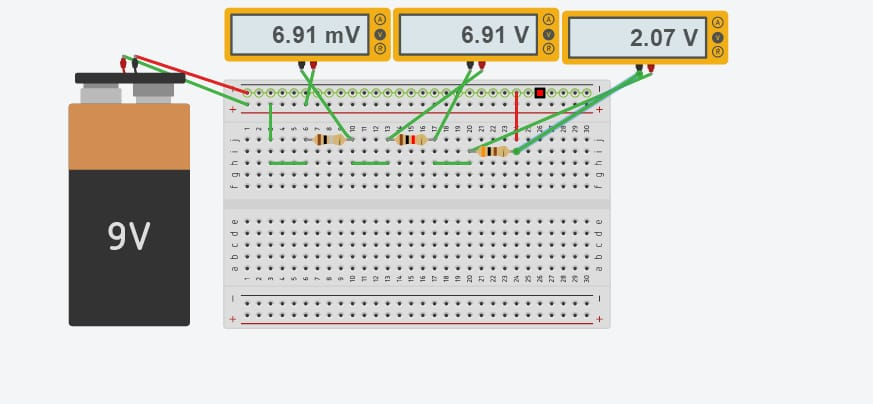
\includegraphics[width=12cm, height=6cm]{g1.png}
			\end{center}
				\end{figure}
\begin{figure}
	\begin{center}
		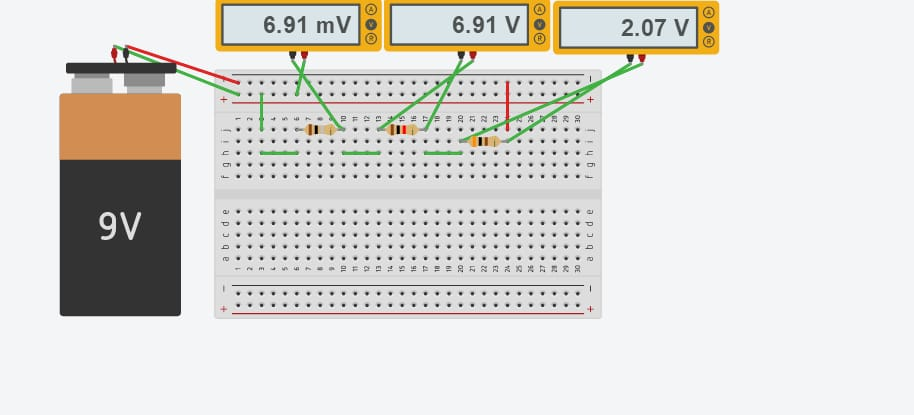
\includegraphics[width=12cm, height=6cm]{g2.png}
			\end{center}
				\end{figure}
\newpage
\begin{figure}
	\begin{center}
		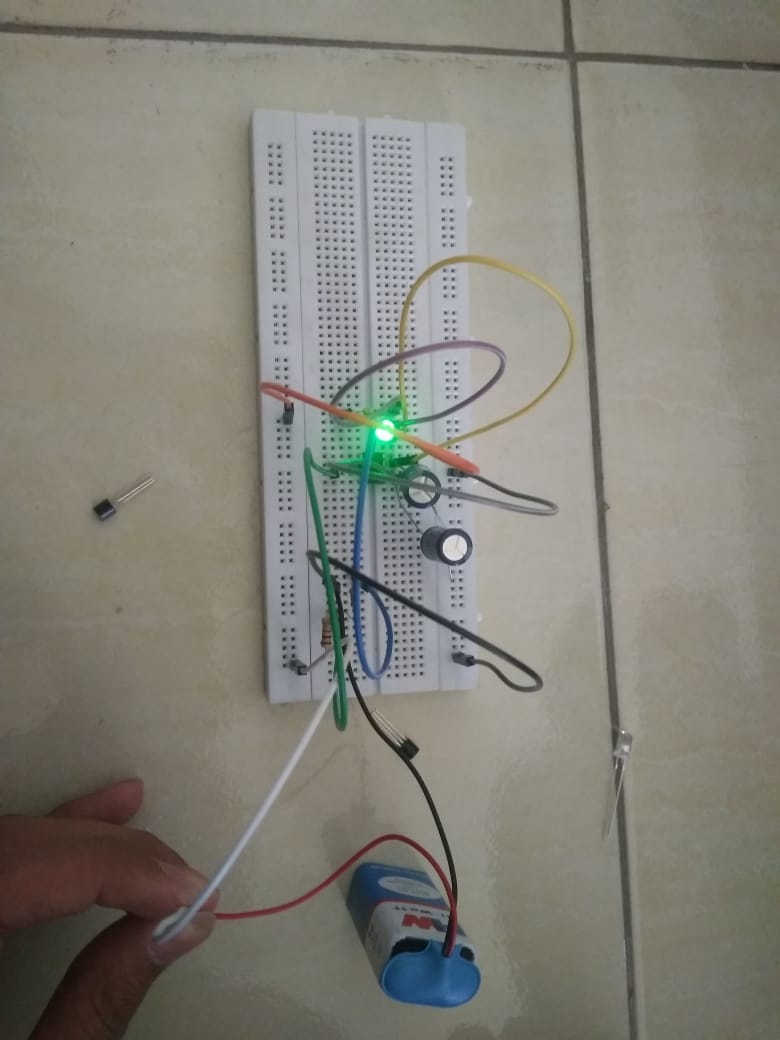
\includegraphics[width=12cm, height=6cm]{g3.png}
			\end{center}
				\end{figure}
\begin{figure}
	\begin{center}
		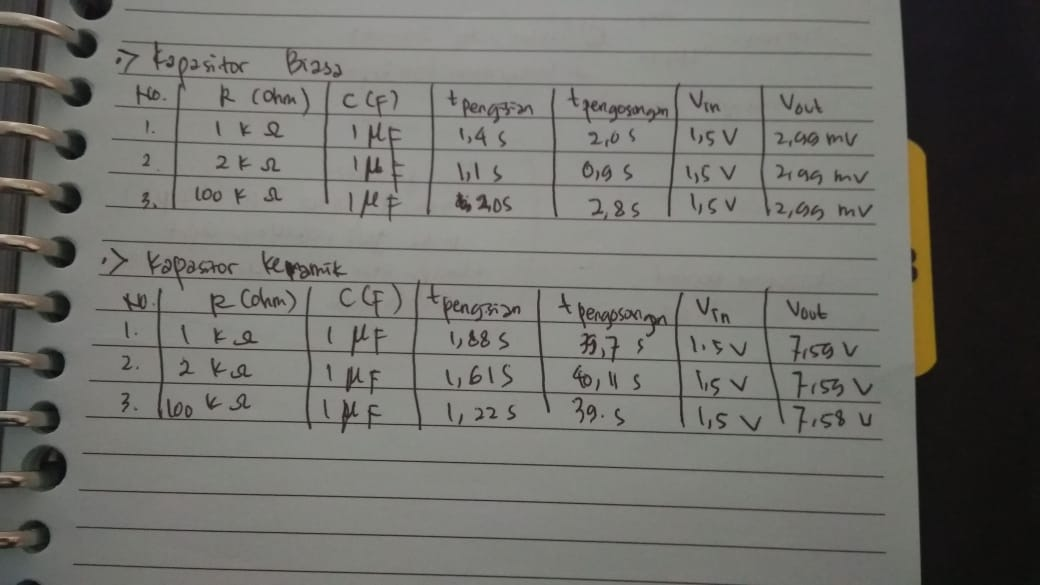
\includegraphics[width=12cm, height=6cm]{g4.png}
			\end{center}
				\end{figure}
\newpage
\begin{figure}
	\begin{center}
		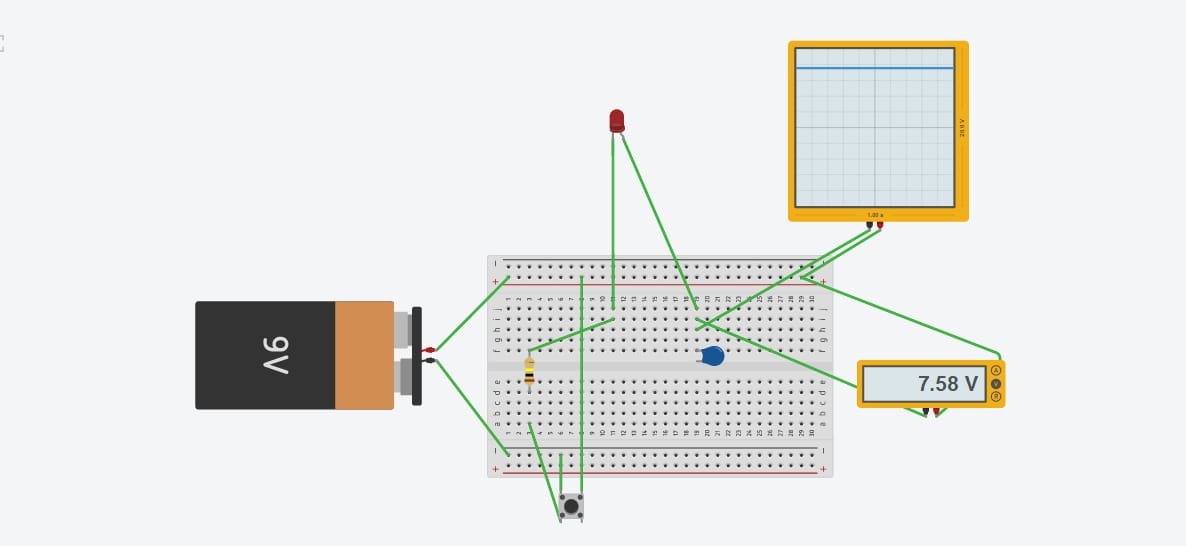
\includegraphics[width=12cm, height=6cm]{g5.png}
			\end{center}
				\end{figure}
\begin{figure}
	\begin{center}
		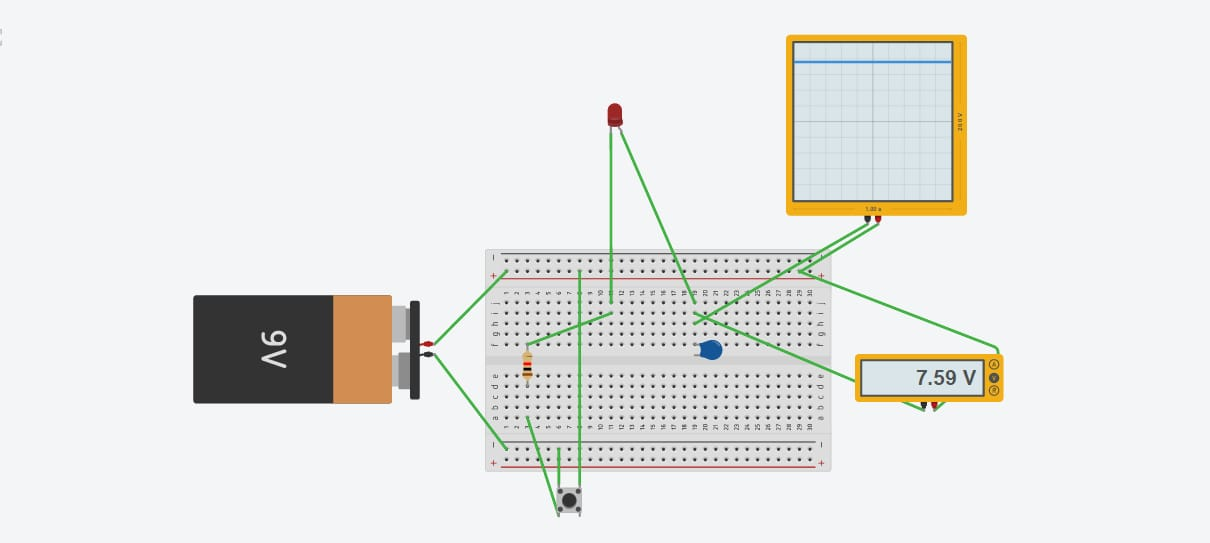
\includegraphics[width=12cm, height=6cm]{g6.png}
			\end{center}
				\end{figure}
\newpage
\begin{figure}
	\begin{center}
		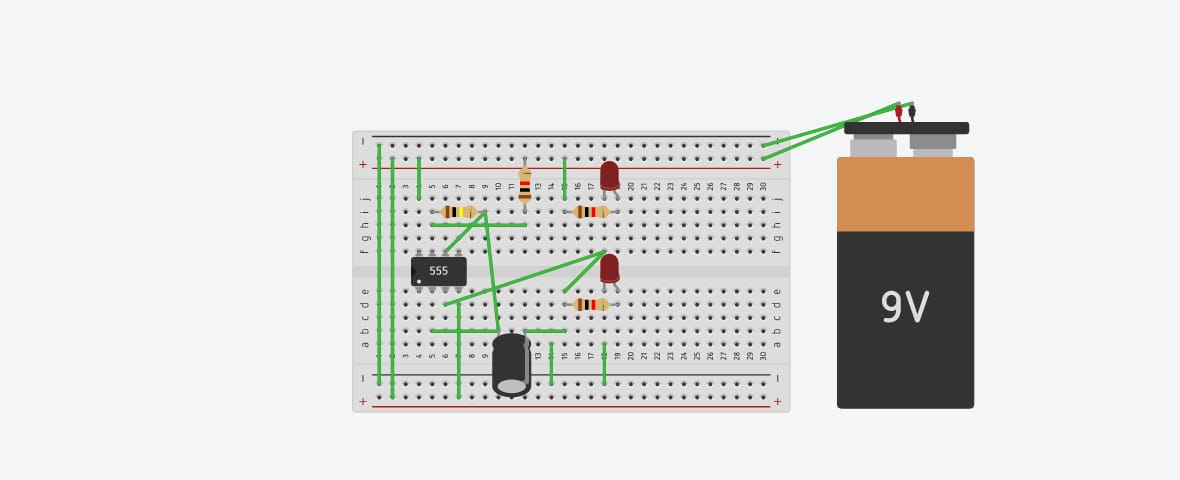
\includegraphics[width=12cm, height=6cm]{g7.png}
			\end{center}
				\end{figure}
\begin{figure}
	\begin{center}
		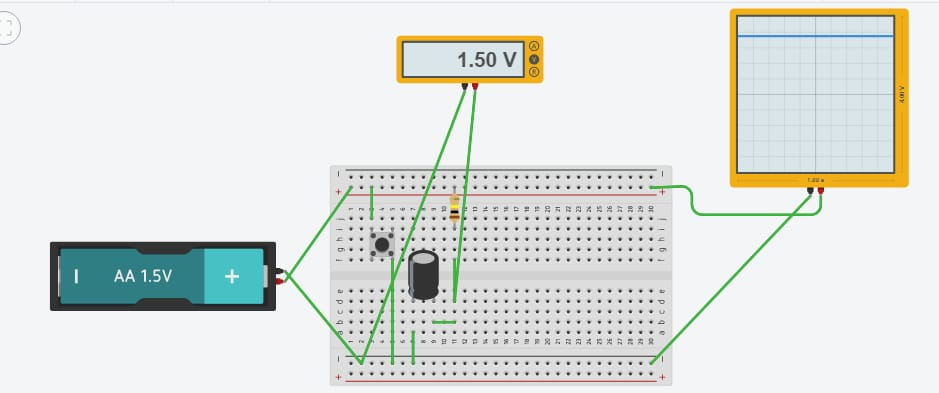
\includegraphics[width=12cm, height=6cm]{g8.png}
			\end{center}
				\end{figure}
\newpage
\begin{figure}
	\begin{center}
		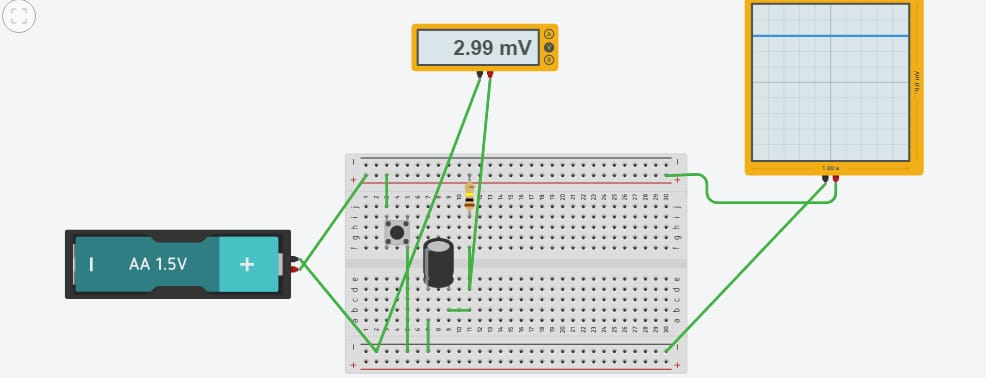
\includegraphics[width=12cm, height=6cm]{g9.png}
			\end{center}
				\end{figure}
\begin{figure}
	\begin{center}
		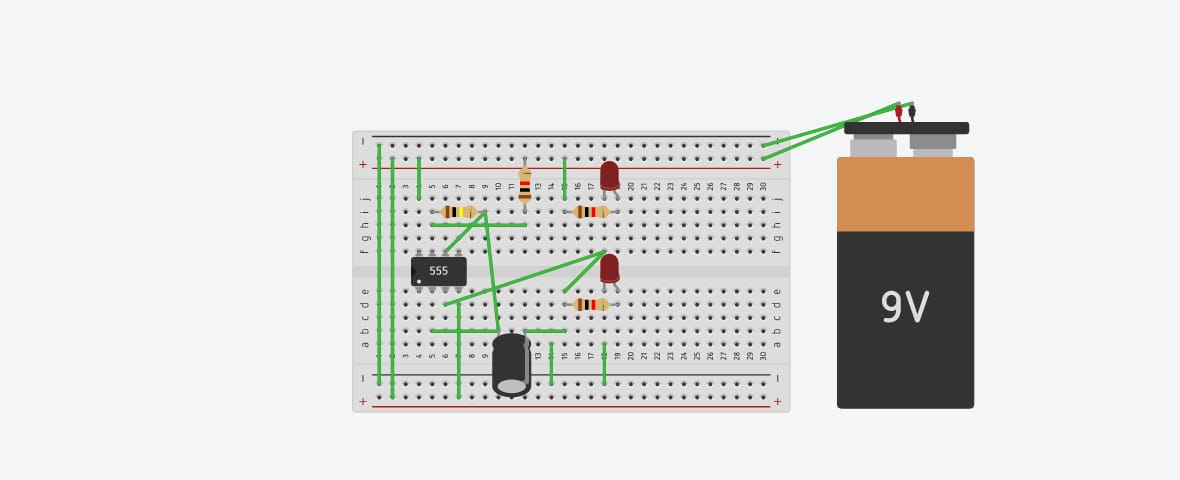
\includegraphics[width=12cm, height=6cm]{g10.png}
			\end{center}
				\end{figure}
\begin{figure}
	\begin{center}
		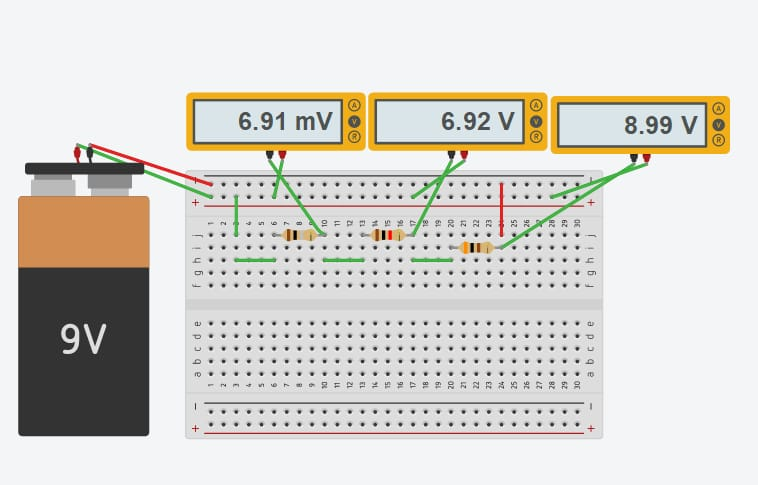
\includegraphics[width=12cm, height=6cm]{g11.png}
			\end{center}
				\end{figure}
				
\end{document} %Penulisan Laporan Berakhir
